\chapter{The Proxima prototype} \label{chap:prototype}

\bc TODO

Bastiaan vragen over v10 types
\ec

% Reuse from Ch_EditModel

A prototype of the Proxima editor has been implemented in the fuctional language Haskell. The architecture of the prototype corresponds to the architecture described in Chapter~\ref{chap:proxArch}, and is realized with the architecture combinators from Chapter~\ref{chap:archCombs}. The implementation is platform-independent and has been succesfully tested on Windows, Linux, and MacOS X platforms. 

The prototype is implemented entirely in Haskell and uses the wxHaskell~\cite{leijen04wxHaskell} library for the implementation of the user interface. The presentation sheet \bc (which is an atttibute grammar)\ec  is compiled by an  attribute-grammar system~\cite{swierstra04ag}, which is also used to implement the arrangement mapping. The parsing sheet is specified using a parser-combinator library~\cite{swierstra01parsers}.

% size of editor?

Proxima is an editor generator, which means that given a document type definition and number of sheets, the system generates an editor application. In the near future, it will be possible to dynamically update the sheets, and hence modify the presentation during editing. In theory, it is also possible to support dynamic updates to the document type, and thus eliminate the need for a generation step altogether. However, it is not clear yet whether the advantages of a dynamic document type justify the effort required to support it.

\todo{mention absence of evaluation layer here?}

The prototype does not yet have any support for incrementality. However, because about 90\% 
of the execution time is taken up by the arrangement and rendering layers, and because editing is typically a local process, simple modifications to these two layers yield substantial results. Experiments with such simple modifications have yielded an  increase of about 900\%,
and lead to an acceptable response time for documents of a few pages. For larger documents we need the underlying attribute-grammar compiler to support incremental evaluation.
\todo{check para}

In Section~\ref{sect:sampleEditors}, we show several example editors that have been instantiated in Proxima. Section~\ref{sect:instantiating} discusses the components that are required for instantiating an editor. In Section~\ref{sect:proxImpl}, we go over the implementation aspects for each of the layers. Finally, Section~\ref{sect:protoConcl} presents an overview of future work and concludes.

% switch with implementation of system?
\section{Instantiated editors} \label{sect:sampleEditors}
\todo{mention size of sheets}
Three editors have been implemented with Proxima: a source editor for the functional language Helium~\cite{heeren03helium}; an editor for presentation slides in the style of Microsoft PowerPoint; and a chess-board editor. Because the editors were implemented mainly for demonstration purposes, all three editors are integrated in a single editor instance.

%Because the editors were implemented mainly for testing concepts, . 
%The editor is connected to the Helium compiler to provide type inference during editing.
%Research vehicle, so many combined features in an incomplete editor. The result is a source editor for the functional %language Helium, integrated with powerpoint slide editor and a chess board. 

\subsection{A Helium source editor}



A source editor has been implemented for a subset of the functional language Helium~\cite{heeren03helium}, which is a  Haskell dialect designed for education. The editor already provides most of the functionality that was described in the source-editor use case (see Section~\ref{sect:sourceeditor}). In order to provide type information during editing, the editor is integrated with the Helium type checker. Figure~\ref{heliumMain} contains a screenshot of the Helium editor in action. \todo{meer over Helium?}

% The Helium type checker is an interesting choice, because it vllsfd . Furthermore, much information 
\bc Helium type checker provides Quality of error messages  Integrated with a compiler for type inference. Helium interesting, because complier has good error messages and info, which is hard to convey in a command line . \ec


\begin{figure}
\begin{center}
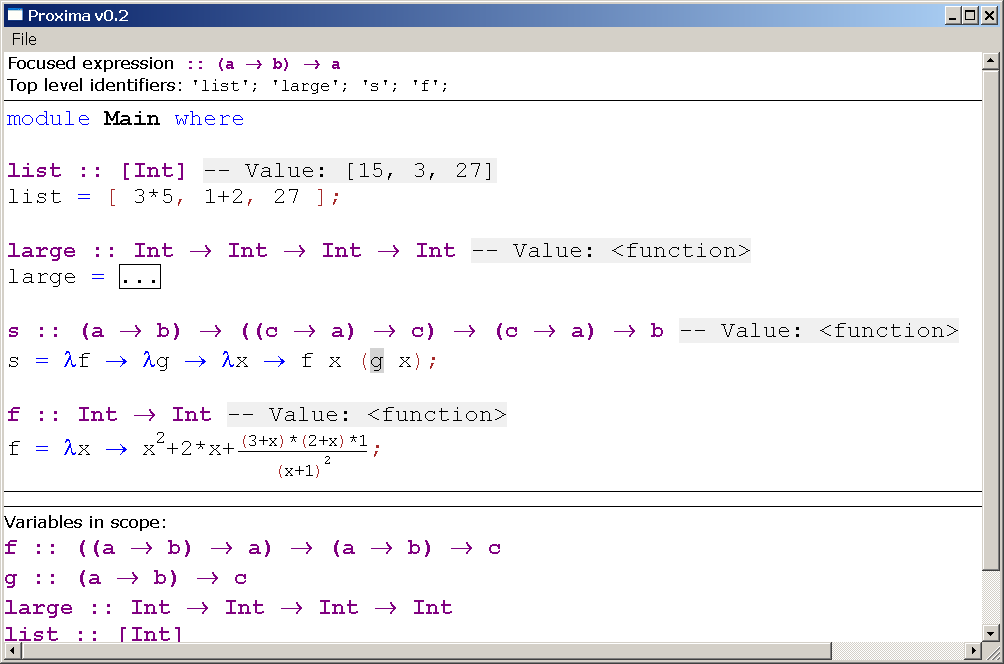
\epsfig{file=pics/Screenshots/heliumWindow.eps, width=10cm}
\caption{An editor for Helium.}\label{heliumMain} 
\end{center}
\end{figure}\todo{focus has wrong color}

In the figure, we see an editable view of a program source, with the focus on \todo{focus}. The right-hand side of function \p{ff} has been hidden and may be expanded by clicking on the dots. The definition of \p{f} shows that program constructs may also have a more graphical presentation.

% semantic coloring, nice arrows?
The type signatures for the top-level declarations are automatically derived. \note{mention these are not editable?} Moreover, the editor provides type information for local expressions as well. At the top of the presentation, we see the type for the document part that is in focus (if it has a type). At the bottom, the variables that are in scope from the focus are listed together with their types.

To the right of each type signature is a comment that shows the value of the declared identifier, which changes dynamically when the source is edited. Although not very useful in a source editor, since most declarations are functions, these computations provide an example of spreadsheet-like behavior; parts of the document that represent computations are interpreted dynamically, and the results are displayed in the presentation.

\head{Presentation-oriented editing mixed with structure editing}

Expressions may be edited structurally (i.e\ document-oriented) based on the Helium abstract syntax. Below is an example that shows how structure editing may facilitate editing a list. When the \p{3*5} element is deleted, the comma next to it automatically disappears. When the element is pasted at the end, a comma appears in front of it. 

%height 30px
\fbox{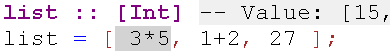
\epsfig{file=pics/Screenshots/strEditList1.eps, height=0.3cm}} \hspace{\stretch{1}}
\fbox{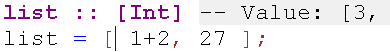
\epsfig{file=pics/Screenshots/strEditList2.eps, height=0.3cm}} \hspace{\stretch{1}}
\fbox{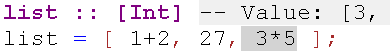
\epsfig{file=pics/Screenshots/strEditList3.eps, height=0.3cm}}
\todo{fix focus and add type sig to screenshot}

Furthermore, the editor supports structure building with placeholders. By selecting constructs from a menu, an expression may be constructed:

%height 60px
\fbox{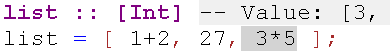
\epsfig{file=pics/Screenshots/strEditList3.eps, height=0.3cm}} \hspace{\stretch{1}}
\fbox{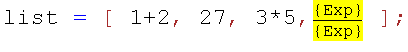
\epsfig{file=pics/Screenshots/strEditBuild2.eps, height=0.5cm}} \hspace{\stretch{1}}
\fbox{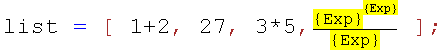
\epsfig{file=pics/Screenshots/strEditBuild3.eps, height=0.5cm}}

Similar structure editing is supported by conventional syntax-directed editors, but Proxima has the advantage that the presentation may still be edited textually as well. Program fragments may be entered or modified textually without having to switch to a different view or mode.  Below is a screenshot that shows a presentation-oriented cut operation. Although the selection that is cut does not make sense at document level, the cut is a valid edit operation at the presentation level.

\begin{center}
\fbox{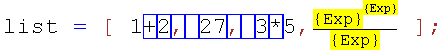
\epsfig{file=pics/Screenshots/presEdit1.eps, height=0.5cm}} \qquad
\fbox{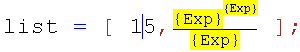
\epsfig{file=pics/Screenshots/presEdit2.eps, height=0.5cm}}
\end{center}

\bc
\begin{center}
\end{center}
\ec

\head{Type errors}

The editor shows type errors by marking the error location with a squiggly line and displaying the error message at the bottom of the source. This mechanism also works in the graphically presented parts of the program, as is shown by the screenshot fragment below.

%\todo{fix (-1,-1)}
\begin{center}
\fbox{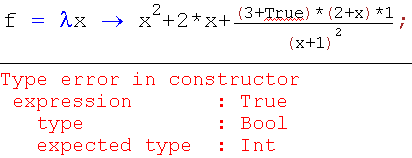
\epsfig{file=pics/Screenshots/typeErr.eps, height=2cm}}
\end{center}

The Helium type checker is an interesting candidate for integration with a structure editor, because of its sophisticated type checker. Besides the location of the error, the type checker can provide additional information about the other parts of the program that contributed to the error. Such information would be hard to show on a command-line, but can be displayed in a clear way by highlighting the relevant parts of the source code. Furthermore, for common errors, the Helium type checker is able to provide hints on how to repair them. Such hints can be presented along with a button that performs the suggested reparation when clicked.


%And no line numbers yet. (but will be easy to add)

%Click on error jumps to source, click on squiggly show error message. The Helium type checker .
%Extra information from tc on error may be shown.

%?\head{Jump to definition}
%
%SCREENSHOT

\head{Beta reduction}

A simple reduction engine may be applied to a term in the source. The screen-shots below show a few steps in the reduction of the application \p{f~3}. First, the function \p{f} is replaced by its definition from Figure~\ref{heliumMain}. Then, a beta-reduction step is performed, and the argument \p{3} is substituted for all (free) occurrences of \p{x} in the fraction. The process may be continued by reducing the mathematical operators, until we get the final value \p{16}.

\fbox{\epsfig{file=pics/Screenshots/beta1_170x90.eps, height=0.8cm}} \hspace{\stretch{1}}
\fbox{\epsfig{file=pics/Screenshots/beta2_500x90.eps, height=0.8cm}} \hspace{\stretch{1}}
\fbox{\epsfig{file=pics/Screenshots/beta3_410x90.eps, height=0.8cm}}

The reduction engine is implemented by an attribute grammar of about 150 lines, which may be reduced further to about 100 lines, once the underlying attribute-grammar system supports default attribute declarations.

Besides illustrating reduction algorithms, source-to-source transformations can be used to implement refactoring operations~\cite{reinke03refactoring}. Furthermore, by inserting the transformed term below the original, instead of replacing it, we can use the editor for creating derivations semi-automatically (e.g.\ in a proof editor).

%\head{Automatic layout}
%?
%SCREENSHOT


\head{Editable list of top-level identifiers}

The evaluation layer has not been completely realized yet, but nevertheles a few experimental evaluation layer features have been implemented. The list of top-level identifiers at the top of Figure~\ref{heliumMain} may be compared to an editable table of contents. Editing the names in the list causes updates to the identifiers in the corresponding declarations, and moving the identifiers results in moving the declarations.

\toHere
%SCREENSHOT
% ""     "after entering ``..'' "      "
\fromHere


\head{Tree view}

A second experimental feature is a built-in tree presentation of the document. The tree is not fully editable yet.

\begin{center}
\fbox{\epsfig{file=pics/Screenshots/treeview.eps, height=3cm}}
\end{center}

Because of the complexity and size of the tree presentation, more support for incrementality is necessary to make it useful. Furthermore, the tree should be displayed in a separate (scrollable) window or window-pane, which is currently not possible in {\Xprez}.

%SCREENSHOT
\todo{XML}
%No tree funct. yet, need some es support. Also xml is not editable because requires different scanner.


\subsection{A poor man's PowerPoint}

Integrated with the Helium editor is a very basic slide editor in the style of Microsoft's PowerPoint. A slide presentation is a list of slides, each of which consists of a title and a list of items. An item is a string, a Helium expression, or a nested item list. Figure~\ref{slideEditorWYSIWYG} shows the slide editor for a slide presentation of two slides. An item list may choose from several display styles (bulleted, numbered, or enumerated with letters) and nested lists get a smaller font size.

Because a WYSIWYG view is not always convenient, the editor also provides an XML view, which is shown in Figure~\ref{slideEditorSource}. The source view is only partially editable, but it is straightforward to turn it into a fully-editable\todo{-?} view. \todo{built-in XML pres?}

\begin{figure}
  \begin{minipage}[t]{.47\textwidth}
    \begin{center}   
\fbox{\epsfig{file=pics/Screenshots/powerpointPresWindow.eps, height=5cm}}
      \caption{Slide editor WYSIWYG view.} \label{slideEditorWYSIWYG}
    \end{center}
  \end{minipage}
\hfill
  \begin{minipage}[t]{.47\textwidth}
    \begin{center}  
\fbox{\epsfig{file=pics/Screenshots/powerpointEditWindow.eps, height=5cm}}
      \caption{Slide editor XML view.\hspace{1cm}} \label{slideEditorSource}
    \end{center}
  \end{minipage}
\end{figure}
\todo{change Helium expression}

\head{Integration with Helium editor}

The slide editor is fully integrated with the Helium editor: a list of slides forms part of the program source, and, more interestingly, a slide may contain Helium code (which may again contain a list of slides, and so on). Moreover, the Helium code in a slide has exactly the same edit functionality as in the source editor. As an example, the screenshot below shows a slide that contains a Helium expression with a type error.

\begin{center}
\fbox{\epsfig{file=pics/Screenshots/powerpointTypeErr.eps, height=3cm}}
\end{center}


\subsection{Chess board}

Altough it might seem a somewhat unfamiliar application of structure editing, a chess board editor lends itself very well to be implemented with Proxima.  Figure~\ref{chessBoard} shows the chess board editor, which is integrated with the Helium editor similar to the slide editor (except that we cannot use Helium expressions as chess pieces).

\begin{figure}
\begin{center}
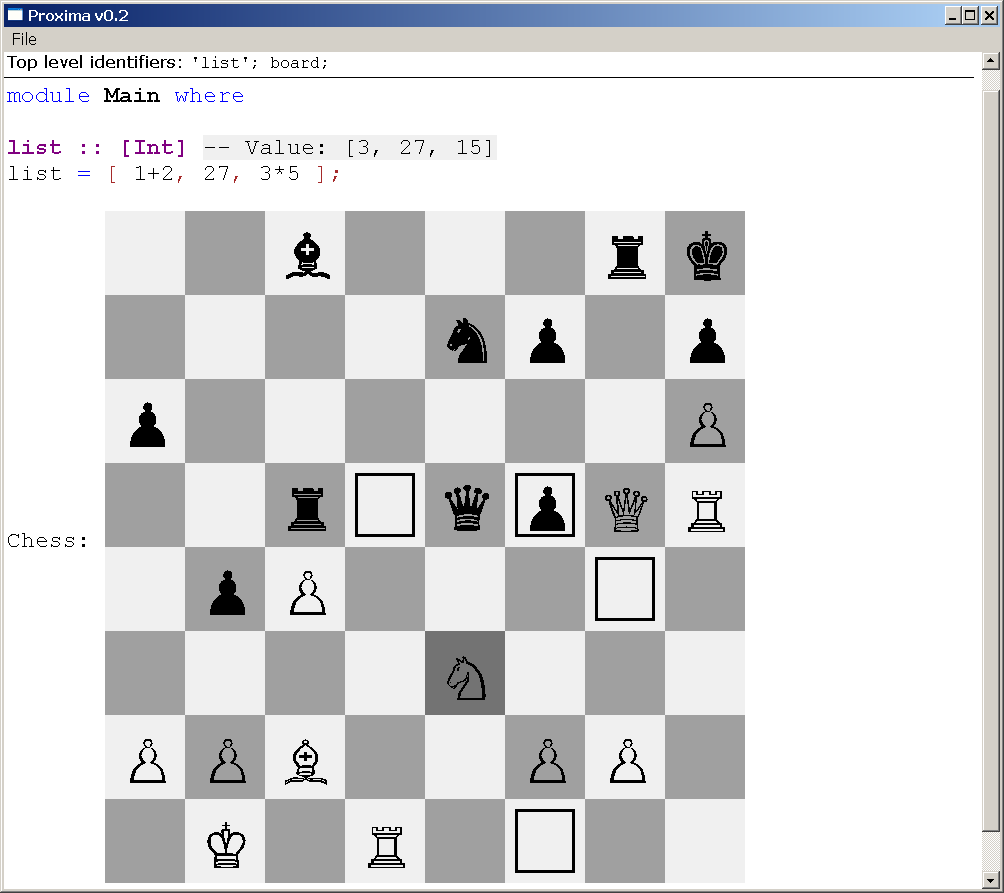
\epsfig{file=pics/Screenshots/chessWindow.eps, height=5cm}
\caption{A chess board editor.}\label{chessBoard} 
\end{center}
\end{figure}

The chess-board editor highlights all squares that are reachable by the focused chess piece. A piece may be moved by clicking one of these highlighted squares, or by using cut-and-paste. The editor does not yet support playing against the computer, but this can be implemented straightforwardly by connecting the editor to a chess program. \todo{forward ref to sheet example?}



%																
%																
%																
\section{Instantiating an editor} \label{sect:instantiating}

In order to intantiate an editor in Proxima, three components need to be provided: a {\em document type definition}, a {\em presentation sheet}, and a {\em parsing sheet}. We will give brief overview and a few example fragments of each of these three components. The {\em evaluation sheet}, {\em reduction sheet}, and {\em scanning sheet} that were mentioned in Section~\ref{sect:archProximaLayers} are not yet fully supported and therefore not discussed here.

Because the sheet formalisms are still in an experimental stage, . \toHere
Still in experimental stage. leave out details that will be hidden in future impl.
\fromHere

\subsection{Document type}

As mentioned in Section~\ref{sect:docLevel}, a Proxima document type consists of monomorphic data types and the list type. The type definition is similar to a Haskell type definition, with a few differences. A constructor may have named children, which do not have to be globally unique. Thus, a binary tree type can be defined as:\todo{name is optional}

\p{data Tree = Bin left::Tree right::Tree | Leaf val::Int}

Furthermore, each constructor needs to specify how many tokens it uses in its presentation. This information can be deduced from the presentation sheet, but, for the moment, it has to be specified by hand. The tokens are specified by a list of children of type \p{IDP} that is enclosed by braces. The special syntax is necessary because Proxima provides default behavior for these types. \todo{id may be new} \todo{also possible list}
%monomorphic (i.e.\ parameter free) data types together with the list type
%\note{comments on generation here or in impl?}

Figure~\ref{docTypeExample} shows several fragments of the document type for the editors from Section~\ref{sect:sampleEditors}.\todo{find out which types to show} \todo{extra state?} \todo{boxed primvals}
\p{Decl} has intr es as and \p{layout} \p{exp} is what? should be hidden


\todo{check that idD is not in figure, types with ::}
\begin{figure}
\begin{small}
\begin{center}
\begin{footnotesize}
\begin{verbatim}
data Root = Root decls::[Decl]

data Decl = Decl exp::Bool_ layout::Bool_ Ident Exp { idP0, idP1, idP2, idP3 }
          | BoardDecl Board                         { idP0, idP1 }
          | PPPresentationDecl PPPresentation       { idP0, idP1 }

data Exp = PlusExp exp1::Exp exp2::Exp              { idP0 }
         | DivExp exp1::Exp exp2::Exp               { idP0 }
         | LamExp Ident Exp                         { idP0, idP1 }
         ...
         | LetExp [Decl] Exp                        { idP0, idP1 }
         | BoolExp Bool_                            { idP0 }
         | IntExp Int_                              { idP0 }

...

data Board    = Board    r1::BoardRow r2::BoardRow r3::BoardRow r4::BoardRow
                         r5::BoardRow r6::BoardRow r7::BoardRow r8::BoardRow { }

data BoardRow = BoardRow ca:Square cb:Square cc:Square cd:Square
                         ce:Square cf:Square cg:Square ch:Square { }

data Square = Square Piece

data Piece = King color : Bool_ { } | Queen color : Bool_ { } | ... | Nothing { }
\end{verbatim}
\end{footnotesize}
\caption{A Proxima document type definition.}\label{docTypeExample} 
\end{center}
\end{small}
\end{figure}
\note{caption}

\bc
         | TimesExp  exp1::Exp exp2::Exp                     { idP0::IDP }
         | PowerExp exp1::Exp exp2::Exp                      { idP0::IDP }
         | AppExp exp1::Exp exp2::Exp                        { }
         | CaseExp Exp alts::[Alt]                          { idP0::IDP, idP1::IDP }
         | IfExp exp1::Exp exp2::Exp exp3::Exp                { idP0::IDP, idP1::IDP, idP2::IDP }
         | IdentExp Ident                                  { }
         | ParenExp Exp                                    { idP0::IDP, idP1::IDP }
         | ListExp exps::[Exp]                              { idP0::IDP, idP1::IDP, ids::[IDP] }
         | ProductExp exps::[Exp]                           { idP0::IDP, idP1::IDP, ids::[IDP] }

-- one pres elt for in program source, other for in list
-- however, only the one for source is used, the other has no layout
data Ident = Ident String_                                 { idP0::IDP idP1::IDP }

\ec

\subsection{Presentation sheet}
\todo{Check swapped hRef vRef  in code}
\todo{If presenter/parser is explained in more detail here, add a forward ref in chapter proxArch}

The presentation sheet is an attribute grammar that specifies the presentation as a synthesized attribute \p{pres~::~Xprez}. Besides the presentation, arbitrary inherited and synthesized attribute may be specified. Furthermore, a number of default attributes is available for each document element.

%Because the sheet is which is directly compiled by an attribute-grammar system.
%The sheet is combined with a generated attribute-grammar module that defines default presentations and ..
%..location.

As explained in Section~\ref{chap:proxArch}, a presentation may be either {\em parsing} or {\em structural}, depending whether or not it allows presentation-oriented editing. If a presentation supports presentation-oriented editing, this is specified in the presentation sheet with the function \p{parsing}. On the other hand, if the presentation is a structural presentation without presentation-oriented editing, we use the function \p{structural}.  The choice between parsing or structural presentations also affects the parsing sheet, as will be explained in the next section. 

To support editing, the presentation should be constructed according to several guidelines, which are not enforced yet. Besides specifying whether it is structural or parsing, a presentation must contain the document location, and change its background color when it is in focus. 

Although the functions for marking the location and presenting the focus are simple, they contain explicit attribute references which require too much detail for this discussion. Because the attribute grammar compiler does not support first-class AG's, we cannot abstract over these functions. Hence, we will denote the two functions by \p{{\em location}} and \p{{\em focus}}. 

\toHere
Difference with \ref{chap:proxArch} is that parsed presentations are not token lists, but just trees.
\fromHere

%$<$$squiggle$$>$ $<$$add~reduction~menu$$>$

We discuss a few presentation examples that originate from the example editors in Section~\ref{sect:sampleEditors}.

\head{Fraction}

The first example is the presentation of a fraction expression in the Helium editor, which makes use of the \p{frac} combinator from Section~\ref{sect:xprezFrac}. A helium expression needs to show a squiggly line when it is the location of a type error and furthermore, it defines a popup menu for beta-reduction edit operations. The two functions that implement this behavior are denoted by \p{{\em squiggle}} and \p{{\em add\_reduction\_menu}}, similar to \p{{\em location}} and \p{{\em focus}}. 

Thus, the presentation for the \p{DivExp} constructor of \p{Exp} is:

\ttfamily\begin{small}\begin{tabbing}
SEM Exp | DivExp\\
~~lhs.pres = ({\em location}~.~structural~.~{\em focus}~.~{\em squiggle}~.~{\em add\_reduction\_menu})\\
~~~~~~~~~~~~~~~frac @exp1.pres @exp2.pres
\end{tabbing}\end{small}\rmfamily
%DivExp      
%  lhs.pres = loc (DivExpNode @self @lhs.path) $ structural $ presentFocus @lhs.focusD @lhs.path $
%               squiggleRanges @lhs.ranges @lhs.path $ addReductionPopupItems @reductionEdit $
%               frac @exp1.pres @exp2.pres

\head{Lambda}

The second example is the presentation of a Helium lambda expression, such as \verb|\x|$\rarr\!$\verb|x+1|. The presentation uses a function \p{key} to display a string in keyword color (i.e.\ the constant \p{keyColor}): \todo{text has an id}

\begin{small}
\p{key :: IDP -> String -> Xprez}\\
\p{key id str = text id str `withColor` keyColor}
\end{small}

Unlike the fraction, a lambda expression is a \p{parsing} presentation. This means that for the presentation of a lambda node, the tokens of its previous presentation must be reused. The presentation consists of two tokens (``\verb|\|'' and ``$\rarr\!$'') which have identifiers \p{@idP0} and \p{@idp1} (see Figure~\ref{docTypeExample}). To reuse the tokens, these identifiers are passed to \p{key}. If the node has not been presented before, the presentation identities have the \p{FreshIDP} value, and will be replaced by fresh unique id's. \note{mention that parser sets the right idps?}

%However, because (for example, when it was just inserted)  The function \p{{\em reuse}~@idP$n$} returns either %\p{@idP$n$} or if \p{@idP$n$} was not defined, a fresh unique presentation id.

\ttfamily\begin{small}\begin{tabbing}
SEM Exp | LamExp\\
~~lhs.pres = ({\em location}~.~parsing~.~{\em focus}~.~{\em squiggle}~.~{\em add\_reduction\_menu})\\
~~~~~~~~~~~~~~~row [ key @idP0 "\verb|\\|"\\
~~~~~~~~~~~~~~~~~~~, @ident.pres\\
~~~~~~~~~~~~~~~~~~~, key @idP1 "\verb|\|174" `withFont` "symb"\\
~~~~~~~~~~~~~~~~~~~, @exp.pres ] \\
\end{tabbing}\end{small}\rmfamily

Note that the arrow is an arrow symbol in a different font (\p{"symb"}).

%($<$$mark~location$$>$.~parsing~.$<$$present~focus$$>$.$<$$squiggle$$>$.$<$$add~reduction~menu$$>$)\\


\bc  | LamExp      
      lhs.pres = loc (LamExpNode @self @lhs.path) $ parsing $ presentFocus @lhs.focusD @lhs.path $
                   squiggleRanges @lhs.ranges @lhs.path $ addReductionPopupItems @reductionEdit $
                   row' [
                          key (mkIDP @idP0 @lhs.pIdC 0) "\\"
                       --   key (mkIDP @idP0 @lhs.pIdC 0) "l" `withFontFam` "symbol"
                        , @ident.pres
                        , text' (mkIDP @idP1 @lhs.pIdC 1) "" -- trick because "symbol" spaces have wrong width
                          , key NoIDP "\174" `withFontFam` "symbol"
                       -- , key (mkIDP @idP1 @lhs.pIdC 1) "->"
                        , @exp.pres ] 
\ec



%\bl
%\o Figure~\ref{presSheetExample} shows a fragment of the presentation sheet for the Helium editor.
%\o Formatter not yet editable or optimal yet.
%\el
\head{Chess-board square}

A presentation sheet may also specify edit behavior, an example of which is found in the presentation of a square in the chess-board editor. When a square is reachable by the focused piece, it displays a marker (see Figure~\ref{chessBoard}) in front of itself, and specifies an edit operation that moves the focused piece when this marker is clicked. 

We show only the part of the presentation that displays the marker and specifies its edit behaviour. This is done by a function \p{pMove}, which is applied to the rest of the presentation of the square (which is denoted by \p{...}).

The squares of a chess board have an inherited attribute \p{@lhs.possibleMoves} that is a list of the locations to which the focused piece can move. The locally defined \p{pMove} first checks whether the location of the presented square \p{(@lhs.colNr, @lhs.rowNr)} is in this list. The square is not reachable, and \p{pMove} returns  \p{pres} unchanged. On the other hand if the square is reachable, \p{pMove} returns an overlay with a marker (\p{mrk}) in front of \p{pres}. Furthermore, the marker has the edit behavior that on a mouse click, an edit operation \p{(move @pth @focus)} is performed, which cuts the piece at the focused square and pastes it at the location of reachable square.
 
\ttfamily\begin{small}\begin{tabbing}
SEM Square | Square\\
~~lhs.pres = ({\em location}~.~structural)\\
~~~~~~~~~~~~~~pMove (...)\\
~~~~~~~~~~~~~~where pMove pres =\\
~~~~~~~~~~~~~~~~~~~~~~if (@lhs.colNr, @lhs.rowNr) `elem` @lhs.possibleMoves\\
~~~~~~~~~~~~~~~~~~~~~~then overlay [ pres,\\
~~~~~~~~~~~~~~~~~~~~~~~~~~~~~~~~~~~, mrk `withMouseDown` (move @pth @focus)]\\
~~~~~~~~~~~~~~~~~~~~~~else pres\\
\end{tabbing}\end{small}\rmfamily

Because the chess board has its own focus representation, there is no application of \p{{\em focus}}.


% move to conclusions
%The attribute grammar is expressive enough to specify complex presentations.
%\bl
%\o still a lot of code is added by hand. Need nice abstractions
%\el

\bc
\begin{figure}
\begin{small}
\begin{center}
\begin{footnotesize}
\begin{verbatim}
SEM Exp
  | PlusExp
      lhs.pres = loc (PlusExpNode @self @lhs.path) $ parsing $ presentFocus @lhs.focusD @lhs.path $
                   squiggleRanges @lhs.ranges @lhs.path $ addReductionPopupItems @reductionEdit $
                   row' [@exp1.pres , op (mkIDP @idP0 @lhs.pIdC 0) "+", @exp2.pres]

| DivExp      
      lhs.pres = loc (DivExpNode @self @lhs.path) $ structural $ presentFocus @lhs.focusD @lhs.path $
                   squiggleRanges @lhs.ranges @lhs.path $ addReductionPopupItems @reductionEdit $
                   frac @exp1.pres @exp2.pres
\end{verbatim}
\end{footnotesize}
\caption{Presentation sheet}\label{presSheetExample} 
\end{center}
\end{small}
\end{figure}
\ec

\subsection{Parsing sheet}

The parsing sheet is specified in Haskell, using a parser-combinator library~\cite{swierstra01parsers}. The parsers take a presentation tree as input. 

Because a presentation may consist of parsing and structural parts, which need to be treated differently, the parsing sheet consists of two different kinds of parsers. For a {\em structural} presentation, we need to specify a {\em recognizer}, which is a very basic parser that follows the structure of the presentation. On the other hand, for a {\em parsing} presentation, we specify a regular combinator parser. 

If a document node has interpretation extra state, not all of its children are in the presentation. Hence, the parser will not have enough information to construct the node. In that case, we use the information from the parsed tokens to determine which document node . In case a node of the right type and constructor is found, we use this node to determine the values of missing children. Because the syntax of reusing may be somewhat confusing without additional explanation, we use a special notation for reusing: if we  construct a value with a constructor \p{Constr} that takes $n$ children, and we wish to reuse the $i$-th child, this is denoted as:

\begin{small}\p{{\em reuse} (Constr child$_1$ \dots {\em child$_i$} \dots child$_n$)}\end{small}
\note{reuse also takes tokens as args}


We briefly discuss the basic notation for parsers.  The \p{<*>} combinator composes two parsers sequentially, yielding a parser that succeeds only if both its component parsers succeed. Further, to combine the results of a number of sequentially composed parsers, we use the \p{<\$>}, 
which is best explained with an example. Consider a constructor \p{Cnstr c$_1$ \dots c$_n$ :: T} and assume that for each of the $n$ children, we have parser \p{parser$_i$}. Now we can construct a parser for \p{T} by using \p{<\$>} to apply a function that constructs ........
\fromHere

\ttfamily\begin{small}\begin{tabbing}
~~~~~~~~~~~ (\verb|\|c$_1$ ... c$_{n}$ -> Cnstr$_1$ c$_1$ ... c$_{n}$)\\
~~~~~~~~<\$> parser$_{1}$ <*> parser$_{1}$ <*> ... <*> parser$_{n}$ \\
%~~~~<|>\\
%~~~~...\\
%~~~~<|>~~~~  (\verb|\|c$_1$ ... c$_{m_n}$ -> {\em reuse}  (Cnstr$_1$ c$_1$ ... c$_{m_n}$))\\
%~~~~~~~~<\$> parser$_{n,1}$ <*> parser$_{1,1}$ <*> ... <*> parser$_{n,m_n}$ \\
\end{tabbing}\end{small}\rmfamily

Thus, we can construct parsers for each alternative of \p{T}, which can be combined with the choice combinator \p{<|>}, yielding a parser for \p{T}. For more information, the reader is reffered to \cite{swierstra01parsers}.

%\o \p{reuse... [tokenNode tk] Nothing (Just \$ tokenIDP tk) (Just t) (Just e))}
We present an example of a parser, followed by two recognizer examples.

\head{Declaration parser}

A declaration (\p{Decl}) may be a Haskell declaration, a slide presentation, or a chess board. If it is a Haskell declaration, we distinguish a normal declaration from a collapsed one, which has ``\p{...}'' for its right-hand side. Thus, we get four alternatives. Furthermore, a Haskell declaration may be preceded by a generated type signature, which is recognized by a function \p{recognizeTypeDecl}.

The declaration parser combines the four alternatives with the choice combinator \p{<|>}. For a collapsed function, the presentation does not contain a right-hand side \p{Exp}, which must therefore be reused. 

\ttfamily \begin{small} \begin{tabbing}
parseDecl = (\verb|\|tkSig idnt tk1 exp tk2 -> {\em reuse} (Decl tkSig tk1 tk2 idnt exp))\\
~~~~~~~~<\$> recognizeTypeDecl\\
~~~~~~~~<*> parseIdent <*> pKey "=" <*> parseExp <*> pKey ";"\\
~~~~<|>~~~~ (\verb|\|tkSig idnt tk1 tk2 -> {\em reuse} Decl (tkSig tk1 tk2 idnt {\em Exp}))\\
~~~~~~~~<\$> recognizeTypeDecl\\
~~~~~~~~<*> parseIdent <*> pKey "=" <*> pKey "..."\\
~~~~<|>~~~~~(\verb|\|tk board -> {\em reuse} BoardDecl (tk board))\\
~~~~~~~~<\$> pKey "Chess" <* pKey ":" <*> recognizeBoard\\
~~~~<|>~~~~~(\verb|\|tk slides -> {\em reuse} PPPresentationDecl (tk slides)\\
~~~~~~~~<\$> pKey "PPT" <* pKey ":" <*> recognizePPPresentation
\end{tabbing} \end{small} \rmfamily
\note{mention typing ``\p{...}''?}

%                                                              -- IDD  "="                   ";"                       type sig
%              not used  expanded    auto-layout
%reuseDecl [tokenNode tk1, tokenNode tk2] Nothing (Just $ tokenIDP tk1) (Just $ tokenIDP tk2) 
%(typeSigTokenIDP sig) Nothing (Just $ mkBool_ True) Nothing (Just ident) (Just exp))
%reuseDecl [tokenNode tk1, tokenNode tk2] Nothing (Just $ tokenIDP tk1) Nothing (typeSigTokenIDP sig)
% Nothing Nothing Nothing (Just ident) Nothing)--makeDecl' mtk0 tk1 tk2 ident) 


%recognizeExp' = pStr $ 
%         (\str e1 e2 -> reuseDivExp [tokenNode str] Nothing Nothing (Just e1) (Just e2))
%     <$> pStructural DivExpNode
%     <*> recognizeExp


\head{Slide recognizer}

A recognizer is specified by a parser that is transformed by the combinator \p{pStr}. The parser part consists of parsers for each constructor of the type, which are combined by \p{<|>} combinators. Each alternative consists of recognizers (or parsers) for each of the children of the constructor, preceded by a special parser that \todo{hoe leggen we dit uit?} For a constructor $Constr$, this special parser is denoted by  \p{pStructural $Constr$Node}.

A slide contains a title string and a list of items.  The title is parsed with the primitive \verb|parseString|. The item lists is recognized by \p{recognizeItemList}.

\ttfamily\begin{small}\begin{tabbing}
recognizeSlide = pStr \$\\
~~~~~~~~(\verb|\|str title itemList -> {\em reuse} (Slide title itemList))\\
~~~~<\$> pStructural SlideNode <*> parseString\verb|_| <*> recognizeItemList
\end{tabbing}\end{small}\rmfamily
%reuseSlide [tokenNode str] Nothing (Just title) (Just itemList))

Because recognizers follow the presentation structure exactly, a future version of Proxima will most likely generate them automatically from the presentation sheet. 
\bc \\
      ((\verb|\_| -> initBoard) <\$> pKey "board")\\
  <|>    \ec
\head{Slide recognizer}

If all descendents of a node have structural presentations, and thus may not be edited at the presentation-level, a recognizer for that node is simple. In this case, the presentation of a node will not have been modified, and instead of descending into the presentation structure, we may simply reuse the node and all of its children.

Hence, the recognizer for the chess board is:

\ttfamily\begin{small}\begin{tabbing}
recognizeBoard = pStr \$\\
~~~~~~~~(\verb|\|str -> {\em reuse} (Board {\em BoardRow} {\em BoardRow} ... {\em BoardRow})\\
~~~<\$> pStructural BoardNode\\
\end{tabbing}\end{small}\rmfamily





%																
%																
%																
\section{Prototype implementation} \label{sect:proxImpl}

%Mappings. no eval.  arr + ren not nec. layout automatic, so only at pres layer.

%Size of system.

The main components of the architecture are the five layers and together with a user-interface module. 
Each layer has a presentation and an interpretation components, which define defining \p{present} and \p{interpret}. A single architecture module imports all component modules, lifts each pair of \p{present} and \p{interpret} functions to a layer, and connects the layers with the combinators from Chapter~\ref{chap:archCombs}.  In total, the generic part of Proxima consists of about 15,000 lines of Haskell code. 

The layers of Proxima generally correspond to the description given in Chapter~\p{chap:proxArch}. The differences between this description and the implementation are listed in the overview of future work in  Section~\ref{sect:protoConcl}.

\subsection{Genericity}

Internally, a document is represented by a Haskell type. Because Haskell is not a generic language, this entails that after changing the document type, those parts of the editor that depend on the document type need to be recompiled. Altough it would be possible to represent a document with an untyped tree structure, we choose a typed implementation because it provides type-safety for the presentation and computation sheets, and also allows a more efficient implementation.

Type specific code is currently generated by a generator written in Haskell. Although lacking safety and transparency, this method does provide the flexibility that we need in this developmental stage of the Proxima project. 

An alternative to the Haskell Generator is the language Generic Haskelll~\cite{clarke02genericHaskell}. However, not all required functions and data types can be described elegantly in Generic Haskell yet. Furthermore, because we also need to generate AG code, switching to Generic Haskell will not eliminate the generator.

\note{future? generic AG?}

\subsection{User interface}

The user interface of Proxima is implemented with the wxHaskell library~\cite{leijen04wxHaskell}, which is  an elegant and fast GUI library with enough low-level support to implement the Proxima renderer. The library is based on the wxWidgets library, and parts of it are generated from a wxWidgets binding to the language Eiffel. As a result, it is relatively easy to keep the wxHaskell library up to date with the latest developments of wxWidgets. 
%low maintenance, more chance of continuity (unlike Fudgets, etc)

Several other actively maintained Haskell GUI libraries are powerful enough to implement the renderer. However, these libraries are based either on the GTK library, which is still poorly supported on windows platforms, or on Tcl/Tk, which is portable but slow.

In Proxima, the dependency on the GUI library is limited to only four modules: the renderer module; a module for the type definitions of the renderer; a module for doing font queries; and a module that opens the main editor window and maps GUI events to Proxima edit gestures. Thus, porting the system to a different GUI library requires only little effort. 


%\o   The HTk, TclHaskell, FranTk and Yahu are based on Tcl/Tk. The Tcl/Tk backend are portable but slow. 
%\o The Gtk+HS, Gtk2HS (no doc),             iHaskell, are based on GTK. Poor windows. 
%Proxima is user-friendly and more appropriate for 90\% of people using windows, than for vi users on Unix etc.
%\o Object I/O is not powerful enough
%\o External renderer was too slow and harder to communicate with. (already mentioned)
%\o integrated in Haskell, much easier than external
\todo{mention Xander van Wiggen for his Renderer?}

\bc
\subsection{The layers}
\toHere

In this section, we only discuss a few interesting aspects of the layers, as well as points where the implementation deviates from the description of mentioned chapter.

\bl
\o Evaluation layer is where document editing takes place. 
\o Doc editing is done with code generation (Only explicit tree editing, presentation-oriented doc editing is done by parsing edited presentation)
\el
%\o Helium type checker is invoked here
%\bl
%\o Layouter is simple. Just process the tree, and add whitespace in the form of spaces and breaks.
%\el
%\bl
%\o AG implements Xprez. with node functions are immediately applied to params.
%\el
\ec


\section{Future work and conclusions} \label{sect:protoConcl}

\todo{Stukje over Haskell?}
\bc
\fromHere
Haskell may not immediately seem the most logical candidate for implementing Proxima, because of statefulness of the architecture; every layer has its own state, and moreover, levels may point to each other. However the architecture combinators hide this state well. 
\toHere

Typical haskell thing Laziness maybe not most important. strictness for speed. unevaluated parts of tree must be made explicit anyway. On the other hand Abstr data types good. Proxima is much tree walking. Type safety?

Most important connection to AG and parser tools. AG with Xprez is good for pres spec. The combination of Haskell with an attribute grammar and a parser library is especially useful for the experimental stage of the prototype. Standard patterns can be expressed elegantly using combinators, but at the same time more primitive combinators can be used to specify and experiment with different behavior.
\ec

In the discussion of future development of Proxima, we distinguish straightforward versus more research-oriented  extensions. \todo{word: extensions?} 

\head{Straightforward extensions}

The prototype is in an experimental stage, which means that there is of future work. 
Besides standard functionality such as file handling, a search facility, etc., and basic fixes, we discuss the major .. for each of the layers. The rendering layer is left out of this discussion, because no straightforward extensions are planned for this layer.Even though straightforward, these extensions may still require a substantive amount engineering.


\head{Evaluation}

An evaluation layer has not been fully implemented yet. The main reason for this is that . 

Because the enriched document type is often very similar to the document type, it is a hassle to have to specify it entirely. However, if we put . We thus need a formalism for specifying extensions and perhaps modifications to the document type, from which the enriched document type is generated. Experimenting with the evaluation layer will be awkward until such support is available.

\head{Presentation} 

Many extensions to the \p{Xprez} formalism are desirable. windows, widgets, formatters, and a page model. Although specified on the presentation level, the implementation of these features will take place mainly at the arrangement and rendering layers.

Currently, . Yet, the parsing library that is used has support for correcting errors and thus keeping parse .
\bl
\o Error correcting parser
\o could repair and put error local.
\o However implemented for now as global parse error, because more experience with whitespace etc. is needed.
\el

An extension of lower priority, but nonetheless straightforward is adapting the layer to support dynamically loaded presentation and parsing sheets. Because the presentation and parsing modules are already clearly separated from the other layers, dynamic loading will not require any fundamental changes to the architecture.


\head{Layout} 

The scanner component of the layout layer is a function that traverses the layout tree and tokenizes the parts that are marked for parsing. Because the specification of the tokens is hard-coded in the scanner definition, it is not straightforward to specify a scanner for a language that has different tokens. Instead, we need a parameterizable scanner, that gets its token specifications from a scanning sheet.

\head{Arrangement}

The arrangement layer needs to be updated to support editable formatters. Furthermore, since this layer performs all the size and position computations for the ******
% Formatters require little more work for keeping mappings


\head{Research}

Besides the straightforward extension to the system, there is a multitude of possibilities for future research on Proxima. We mention a few of the most important areas.

\toHere
\begin{description}
\item[Incrementality.] -Probably the most important future research area for Proxima is support for incrementality. Incrementality. easy tricks diffing. other ag stuff. maybe more complex explicit model: only requesting evaluation of what is needed.
\item[Extra state.] -Extra state is supported, but needs + language support  % \o Storing presentation extra state.
\item[Full evaluator layer.] -Language support is needed in order to facilitate the specification of 
\item[Focus model.] Proxima has a concept of focus on the layout level as well as on the document level, and possibly even on the enriched document level. A focus model must be developed to integrate these different kinds of focus and translate one kind to another.
\item[Graph support.] -Basic support for graphs, or at least presentations such as windows file folder with free layout.
\item[Edit formalism.] -Edit commands are specified with the basic cut and paste operations. We need a /combinator library for edit commands
\end{description}

\fromHere
The first thing to do will be the instantiation of more example editors. Especially a word-processing editor will be interesting, because this application has not been researched extensively in Proxima. The instantiations will allow us to prioritize the list of future research, as well as suggest more areas of research. Furthermore, by examining common patterns in the sheets of the intantiated editors, we can determine what the useful abstractions and libraries will be for these sheets.